\chapter{Technical Background} \label{cpt-technical-background}

\section{Voxel Scene Layout}

The voxel rendering in our evaluation relies on a volumetric representation of the scene.
It is particularly important that the voxel model not only includes the surface but also 
the space within the model. This constraint is often used in interactable use cases, where 
the model is split, cut or manipulated in any given way. [@TODO: Reference Minecraft] lets
the player take full control over the sandbox environment and allows adding or substracting 
any voxels. Essentially, the voxel data of every possible voxel within the playable space 
needs to be somehow present or encoded in memory, even though just a fraction of the voxels 
are actually drawn to the screen.\\

\subsection{Three Dimensional Grid} \label{subsec-three-dimensional-grid}

A basic approach for a scene representation is a three dimensional voxel grid. This 
approach relies on a fixed size grid where each grid cell represents one voxel.
To draw the voxels, a seperate buffer can hold additional voxel information, which 
can be accessed by a given grid cell index. The voxel data can store information about 
whether a voxel is present in that particular grid cell or not, which color the voxel 
should have, the normals for lighting calculation and any other data necessary.
This approach is relatively lightweight but inefficent for large grid sizes and low 
grid occupations. All grid cells need to be traversed to draw any given scene. This 
might include a lot of empty grid cells. Additionally, storing the voxel data seperately
introduces a pointer indirection on each step of the traversal, potentially leading to more 
cache misses.

\subsection{Octree Data Structure} \label{subsec-octree-data-structure}

[@TODO: source] proposes the use of a spatial container to optimize traversal. The use of an octree 
incorporates the relevant scene space and subdivides it into smaller child nodes. When inserting data 
into the octree, the position is evaluated and the data is being stored as a \emph{payload} in 
a node which includes the given position. If a node holds more payload instances than a specified threshold 
allows, it is split into eight child nodes and the payload originally present in the node is 
distributed onto the child nodes. This process is repeated until all data is finally inserted 
into the octree. The resulting octree maintains all the relevant payload data, having a deeper tree 
hierarchy where more data is present and a shallow hierarchy where almost no or no data is present.

[@TODO: Mention other spatial containers -> Binary Space Partitioning Trees]

Octrees like this can vary in their specific implementation, especially in how they maintain the 
payload. Some might store it right next to the octree node description, others might want to separate 
octree and payload data. Octree nodes could also be appended to a dedicated buffer and therefore be stored 
seperately to the tree hierarchy description. Such an approach would maintain chache coherency during an 
unordered traversal of all octree nodes. [@TODO: find appropriate sources]

When using hierarchical data structures dedicated vertex positions can be omitted and instead, 
the voxel position in space can be implicitly calculated from the hierarcical structure and the 
root nodes bounds. This allows for improvement of memory occupation, which is vital for loading and 
storing high resolution voxel scenes. A voxels state can be encoded into either visible (1) or empty (0).
A bitwise representation of voxels can significantly decrease the memory footprint which is a concept 
on which the next approach expand on.

\subsection{High Resolution Sparse Voxel Directed Acyclic Graphs} \label{subsec-highres-svo-dags}

Assarsson et al. (\cite{Assarsson2013}) use data redundancy to further generalize and optimize high resolution 
\ac{SVO}s. In their implementation the octree data structure relies on bitmasks, to encode the existance of child 
nodes. This way, empty nodes are ignored and the information can be easily stored within one byte. This child node 
mask uniquely identifies the layout of the nodes below and can also be used to store the voxel occupation of the 
leaf nodes. Next, they make use of the fact, that an octree nodes position is uniquely identifed by the path along 
the nodes from root to leaf node. Since voxels can be encoded as either being present or not, and non-present 
voxels can be ignored, the data can be significantly reduced in size. Furthermore, equal child node masks 
can simply be shared between different parent nodes instead of being duplicated. Assarsson et al. (\cite{Assarsson2013}) 
suggest a buttom-up approach to remove redundant nodes and replace whole sub-trees of the octree by pointing to one 
instance of the same pattern within the tree, which is shown in figure \ref{fig:sparse-voxel-dag-creation}. 
This optimization can be recursively done to each layer in the tree hierarchy, resulting in an optimized version 
of the data structure. The resulting structure is a more general hierarchical data structure, namely a \ac{DAG}.

\begin{figure}[h]
    \centering
    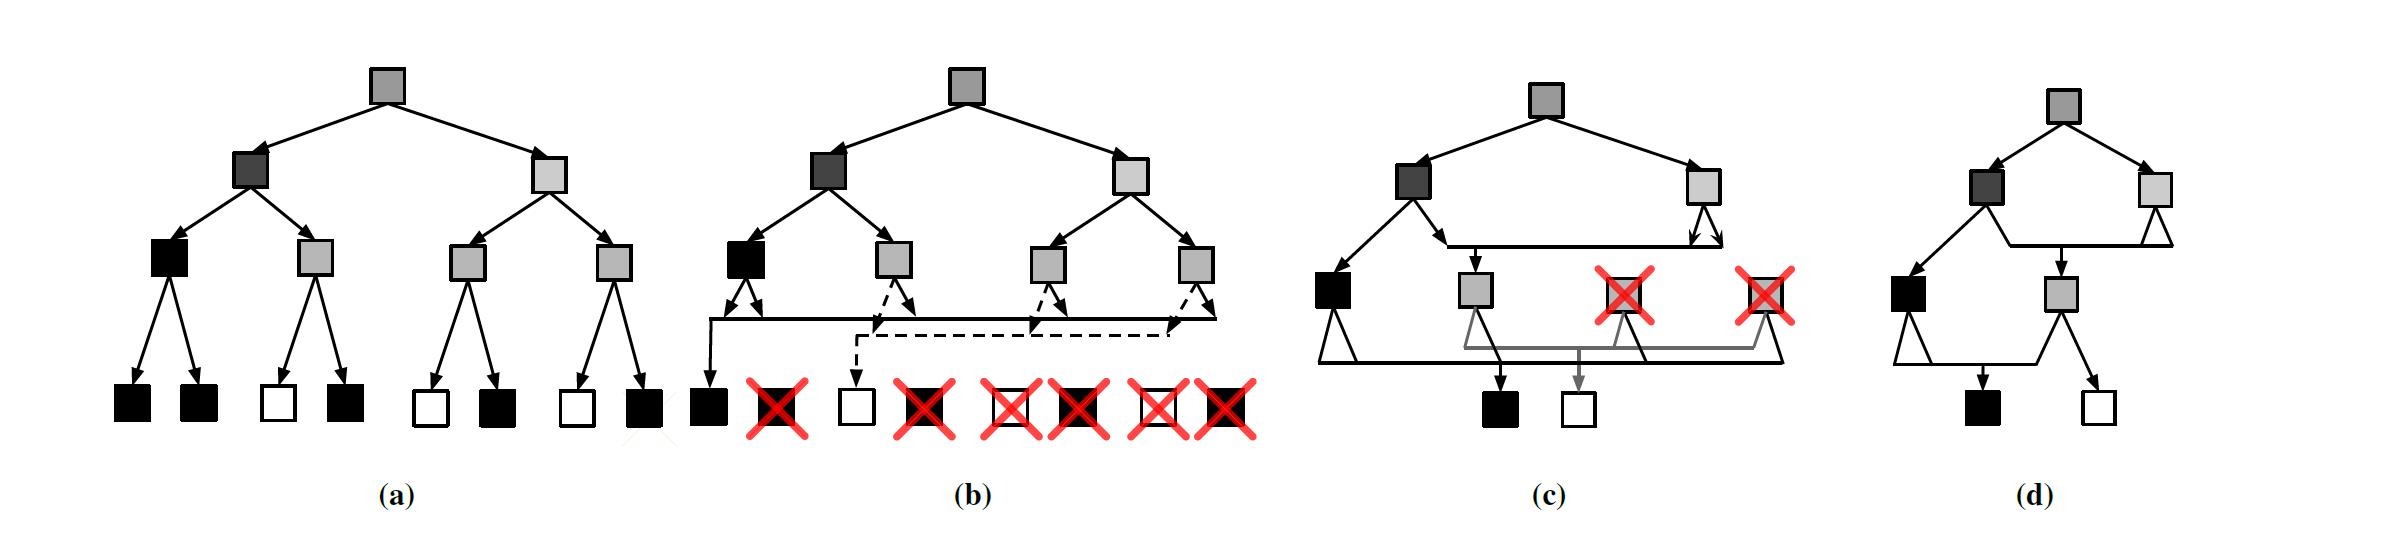
\includegraphics[width=\linewidth]{images/graphics/highres-sv-dag.png}
    \caption{Reducing a \ac{SVO} using the approach of \cite{Assarsson2013}.}
    \label{fig:sparse-voxel-dag-creation}
\end{figure}

This approach seems to be the best solution for reading, storing and optimizing octree data, although we use 
a more basic approach in our implementation. Nevertheless, this concept of optimizing voxel data is compatible 
with our use case and is highly recommended by us.

\section{Culling Techniques} \label{sec-culling-techniques}

\emph{Culling} refers to the technique to discard parts of a scene "that are not considered to contribute to the final 
image" \cite{AkenineMoeller2018}. This allows for a highly populated scenes to be rendered, since most parts of a scene 
will probably not be visible by the camera at the same time. Ignoring culled objects or triangles is therefore a common 
process in realtime rendering. "The fastest triangle to render is the one never sent to the \ac{GPU}" \cite{AkenineMoeller2018}.
In this section, the most common culling techniques are presented and the ones considered by our approach are specifically 
highlighted and analyzed. 


\subsection{Backface Culling} \label{subsec-backface-culling}

Backface culling is probably the most commonly used culling algorithm. It is concerned with discarding triangles which are 
facing away from the camera. These triangles will not be seen by the camera anyway and thus can be safely ignored in the 
rendering process. To compute the facing direction of a triangle, which when normalized is equivilent to the triangles 
\emph{Surface Normal}, the vertex winding order of the given rendering backend is considered.\\

\begin{figure}[h]
    \centering
    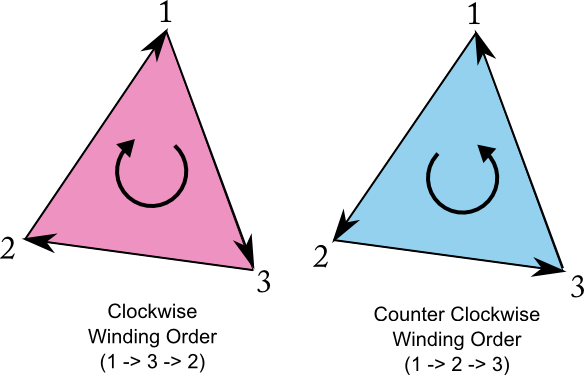
\includegraphics[width=200px]{images/graphics/winding-order-triangle.png}
    \caption{Two possible winding orders of triangles (\cite{Michel2016}).}
    \label{fig:triangle-winding-order}
\end{figure}

\noindent
When describing a triangle mathematically, the vertex positions are considered, which perfectly define the edges of 
said triangle. The surface can then be interpreted as facing towards the viewer or away from them. 
When trying to compute the triangle, its vertex positions can be recorded in an arbitrary order, but to encode which direction 
the surface is facing, the vertex position order is specified up front. Microsoft's rendering \ac{API}s D3D11 and D3D12 for 
example encode a counterclock-wise \emph{winding order} to be interpreted as facing towards the viewer (\cite{D3DTopology2020}).
With this standard in place, all triangles can be uniquely define their orientation relative to the camera.
When enabling backface culling within the renderin backend, triangles which are not facing the camera, are automatically omitted 
immediatly after screenmapping (\cite{AkenineMoeller2018}). Depending on the type of geometry, backface culling can remove up to 
half of the triangles about to be rendered, proving very valuable to highly populated scenes and high geometric density.\\

\noindent 
[@TODO: Add image]
Backface culling algorithms can also be applied to clusters of triangles. As \cite{Shirmun1993} propose, multiple triangles can 
be culled at once considering a common normal cone. "Shirmun and Abi-Ezzi \cite{Shirmun1993} prove that if the viewer is located 
in [a] frontfacing cone" constructed by the normals of all the triangles within the cluster, "then all faces in the cone are 
frontfacing, and similarly for the backfacing cone" (\cite{AkenineMoeller2018}). As will be mentioned in chapter 
\ref{subsubsec-meshlet-backface-culling}, this approach can be used for more parallelized backface culling using an updated 
rendering pipeline in current graphics \ac{API}s.

\subsection{View Frustum Culling} \label{subsec-view-frustum-culling}

[@TODO: Add pictures]

\emph{View Frustum Culling} is a technique which aims to remove instances, i.e. meshes, which are outside of the camera view frustum.
This leads to a descard of all instances which are completely invisible due to their location relative to the camera. Said 
instances can thus be safely ignored and discarded early in order to keep the memory computations by \ac{CPU} and \ac{GPU} low.
To cull potantial instances, bounding boxes are calculated and checked against the camera view frustum, which in turn is specified by 
the \emph{near plane} and \emph{far plane}, as well as the \emph{fov}. For instance, if a bounding sphere is partially or completely 
inside the view frustum can then be tested by computing a simple \boldmath{dot product} between the frustum plane and the bounding volume 
center and comparing it against the radius of the bounding sphere. \\

\noindent
In combination with acceleration structures like an octree, view frustum culling can be computed in for the bounding volumes of the 
acceleration structure which can further optimize the computation. This technique is also applied in our approach, using spheres as 
approximations for the cubical octree bounding volumes.

\subsection{Occlusion Culling} \label{subsec-point-based-occlusion-culling}

When considering highly populated scenes, there might be cases of meshes occluding other meshes. This produces overdraw when rasterizing 
the final projection, which means that multiple color values will be calculated for the same pixel before the final color is determined. 
In general, overdraw should be avoided where possible. Having a lot overdraw within the rendering process means that visibility determination 
of instances is deferred to the last possible point in rendering pipeline. Often, it is better to pre-determine visibility and sample only 
visible instances. Different occlusion culling algorithms can be applied depending on the use case 

\subsection{Hierarchical Z-Buffering} \label{subsec-hierarchical-z-buffering}

\subsection{Two-Pass Occlusion Culling} \label{subsec-two-pass-occlusion-culling}

\section{Mesh Shading}  \label{sec-mesh-shading}

Mesh Shaders were first introduced to NVidia Touring \ac{GPU}s in 2018 as a part of
"a new programmable geometric shading pipeline" and build upon the compute programming 
pipeline (\cite{Kubisch2018}). Therefore, they aim to optimize work by 
using the available hardware more efficiently. Compared to the traditional vertex shading 
pipeline, mesh shading introduces a more holistic and parallel processing of geometry data.
It is incorporated into the rasterized rendering pipeline and has since been used in modern 
gaming. It gained a lot of attention when it was used as the foundation of Epic Games 
Unreal Engine 5 feature \emph{Nanite} [@TODO: source].\\

\subsection{The Mesh Shading Pipeline} \label{subsec-the-mesh-shading-pipeline}

In contrast to the \emph{Mesh Shading Rendering Pipeline}, the "traditional" \emph{Vertex Shading Pipeline} 
has more specialized stages. Figure \ref{fig:traditional-rendering-pipeline} shows all the stages available 
to developers. This pipeline is composed of fixed, programmable and optional stages, where each 
stage operates on some input data and in some cases produces output data for the next stage to consume.\\

\begin{figure}[h]
    \centering
    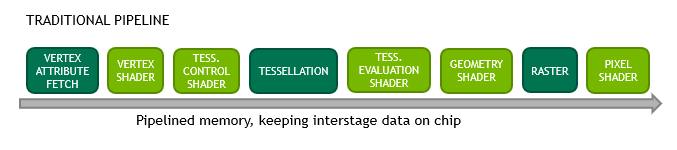
\includegraphics[width=\linewidth]{images/graphics/traditional-rendering-pipeline.png}
    \caption{The traditional rendering pipeline as presented by nVidia in \cite{Kubisch2018}.}
    \label{fig:traditional-rendering-pipeline}
\end{figure}

\noindent
The \emph{Vertex Attribute Fetch} stage (also called \emph{Input Assembler} stage) collects the geometric 
input and creates primitives out of it, reading all necessary data associated with the primitive data. 
These primitives are usually triangles but this can vary slightly from usecase to usecase, depending
on the prior configuration of the stage. After the Input Assembler, the data is sent to the \emph{Vertex Shader}.
This stage is responsible for operating on vertex transformations, moving, rotating, scaling and distorting the 
vertices according to the given transformation matrices. After that, the \emph{Tesselation Control Shader} can 
optionally increase geometric resolution or triangulate polygonal geometry by applying tesselation functions.
The next stage is the optional \emph{Geometry Shader}, which is capable of generating additional primitives 
on the \ac{GPU}. However, it is commonly said to be not very efficient and is treated as deprecated since the introduction 
of the more general purpose and faster \emph{Compute Shaders} [@TODO: source]. 
The three-dimensional scene is then processed by the \emph{Rasterizer} which breaks down the scene description into 
a discrete, two-dimensional "image". This final image, also called \emph{Frame Buffer}, contains the two-dimensional 
projection of the scene from the cameras point of view. This rasterization process also implies creating discrete 
samples from continuous lines and faces.
Finally, the final frame buffer is colored correctly by the \emph{Pixel Shader}. This stage takes all given parameters 
like light position, light color, light intensity, camera position, vertex colors, textures and many more into account 
and creates a final image. The pixel shader can implement different functions (\ac{BRDF}) for calculation of the final 
pixel color and is called once per pixel. This means, that the computational cost increases with the amount of pixel, 
i.e. the frame buffers resolution. 


\begin{figure}[h]
    \centering
    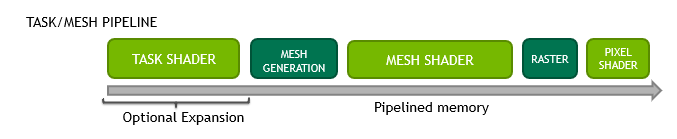
\includegraphics[width=\linewidth]{images/graphics/mesh-rendering-pipeline.png}
    \caption{The mesh shading pipeline as presented by nVidia in \cite[Christoph Kubisch]{Kubisch2018}.}
    \label{fig:mesh-rendering-pipeline}
\end{figure}

The \emph{Mesh Shading Rendering Pipeline} is the a rendering pipeline, optimized for high geometrical 
density. It shares the Rasterizer and the Pixel Shader stages with the Vertex Shading Pipeline but 
introduces two new stages which aim to replace the Vertex Shader, Geometry Shader and Tesselation stage.
The new stages are called \emph{Task Shader} (or \emph{Amplification Shader}) and \emph{Mesh Shader}. Both 
are fully programmable and are based on the Compute Shader architecture. Therefore they are inherently different 
from the traditional Vertex Shader stage, even though they both can be used for vertex transformations.
Figure \ref{fig:mesh-rendering-pipeline} shows the piepline stages and the order they are executed in. \\

\noindent
The Task Shader serves as a precomputational stage which is optional and invokes the Mesh Shader.
The Task Shader can take any arbitrary data as input and operates on the data to produce output data which in 
turn is scheduled for execution on the Mesh Shader. Since both shaders are based on Compute Shaders, a thread 
group size can be specified and groupshared memory can be allocated. This allows for highly parallelized execution 
and optimized memory usage. A key difference to the traditional pipeline is, that the Amplification Shader can 
invoke other compute shaders, create new tasks and dispatch none, one, or multiple mesh shader invocations. This 
makes the shader extremely flexible and capable of providing the same results as the Geometry Shader did.\\

[@TODO: Add picture of meshlets]
\noindent
The Mesh Shader output can be defined individually but usually it creates a small patch consisting of a small 
number of triangles, called \emph{Meshlet}. This new approach to operating on vertices allows for a new interpretation 
of mesh data. The primitive topology is not anymore constrained to triangles, triangle fans and triangle strips, 
but can be individually specified by the developers.
Meshlets are computed by thread groups which usually fetch the mesh data from the given buffers and apply 
transformations and arbitrary operations. This new way of processing geometry is not only more efficient in many cases 
and reduces the memory bandwidth, but also allows for per-meshlet operations (\cite{Kubisch2020}). This is a key 
advantage, since per-instance geometry can now be processed in parallel and still be individually discarded or post 
processed. There are several other advantages over the traditional Vertex Shaded Pipeline, which we will not list to 
the full degree. More details are provided in \cite{Kubisch2020}.\\


\subsection{Meshlet Culling} \label{subsec-meshlet-culling}

One major innovation which is enabled by the use of Mesh Shading is to cull on a per-primitve (per-meshlet) basis. 
This allows for more granular culling of high density geometry even within instances. Prior to the implementation 
of meshlets, culling had to be done on a per-instance basis (or for backface culling on a per triangle basis), 
ommiting whole instances depending on their position in space or their visibility from the point of view of the camera.\\

\noindent
But although the Mesh Shading Pipeline was first introduced in 2018, the idea of triangle clusters goes back even further.
One example of this \ac{GPU} Driven Rendering technique is the 2014 title \emph{Assassin's Creed Unity} (\cite{Ubisoft2014}).
\cite{Aaltonen2015} provides an overview over multiple cluster related optimization techniques, implementing a highly 
parallelized rendering pipeline before Mesh Shading became part of the official Rendering \ac{API}s.
For their \ac{GPU} culling algorithms they refer to the prior work of Hill (\cite{Hill11}) and Greene (\cite{Greene93}) which 
provides the basis for some of the implementation in our case study.


\subsubsection{Meshlet Backface Culling} \label{subsubsec-meshlet-backface-culling}

[@TODO: Rewrite in context of Backface culling above]
Backface culling refers to the discard of triangles, which face away from the camera. These triangles can usually be omitted 
since they will not be seen by the camera anyway. Except from a few exceptions, backface culling can be applied to the 
pipeline configuration safely. Meshlet backface culling refers to the same principle. In this case, not individual triangles  
are culled but whole meshlets are discarded if they are facing away from the camera. Practical algorithms to determine meshlet 
orientation are [@TODO: cite algos].\\ %\cite{} \cite{} \cite{}

%\noindent
%Meshlet backface culling can be more efficient because adjacent triangles usually face in similar directions.

\subsubsection{Meshlet View Frustum Culling} \label{subsubsec-meshlet-view-frustum-culling}

\subsubsection{Meshlet Occlusion Culling} \label{subsubsec-meshlet-occlusion-culling}